\section{Implementation Details - Curvilinear Geometry}
\label{impl-geometry}

\subsection{Analytical Interpolatory Vector}
\label{impl-geometry-analytical-vector}

\noindent
Produces an analytical map from local to global coordinates in terms of polynomial vector. This implementation follows closely the section \ref{theory-lagrange}

\begin{itemize}
  \item 0) Constructs local grid points $\vec{r}_i$
  \item 1) Constructs monomial basis $\vec{z}^{ord}(\vec{r})$
  \item 2) Evaluates all monomials $\vec{z}^{ord}(\vec{r})$ at all local grid points $\vec{r}_i$, assembling the DynamicMatrix V
  \item 3) Computes all lagrange polynomials using $\vec{L}(\vec{r}) = V^{-1} \vec{z}^{ord}(\vec{r})$
  \item 4) Computes the analytical map $\vec{p}(\vec{r}) = \sum_i \vec{p}_i L_i (\vec{r})$.
\end{itemize}

\subsection{Subentity Interpolator}
\label{impl-geometry-subentity-interpolator}

\noindent
Constructs Interpolator classes for each $\dim - 1$ subentity of the given element. Only allowed for elements of dimensions 2 and 3. At the moment a rather crude algorithm is employed. To find the vertices corresponding to a given boundary, the order numbers of simplexGrid are written in a $(ord + 1) \times (ord + 1) \times (ord + 1)$ matrix, which is then used to easier locate the indices of the boundary interpolatory points in the vertex vector. Certain orientation convention is chosen for the provided sub-entitiy interpolators, to simplify the future calculation of the outwards normals. The convention for edge orientations for a triangle $(012)$ are $(01)$, $(12)$ and $(20)$. The convention for triangle orientations for a tetrahedron $(0123)$ are $(012)$, $(023)$, $(213)$ and $(031)$.


\begin{figure}[hp]
    \centering
    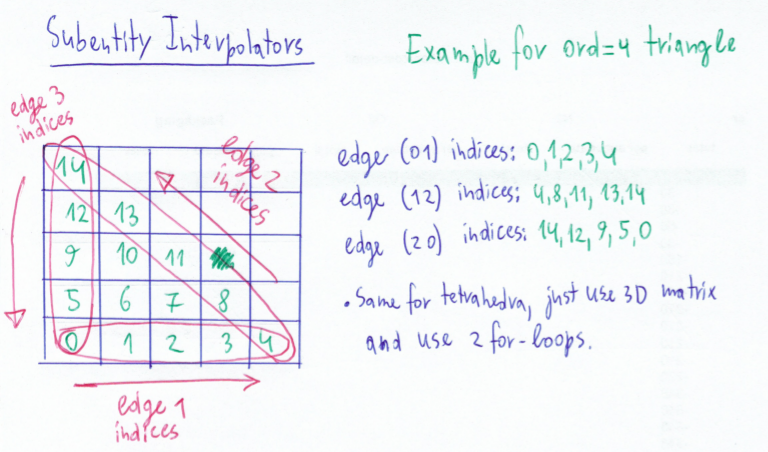
\includegraphics[scale=0.5]{doc-pics/pic-subentity-interpolators-method.png}
    %\caption{Awesome Image}
    %\label{fig:awesome_image}
\end{figure}


\subsection{Local-to-global Mapping}

\subsection{Normals}

\subsection{Analytical Integration}